\documentclass{article}

\usepackage{arxiv}

\usepackage[utf8]{inputenc} % allow utf-8 input
\usepackage[T1]{fontenc}    % use 8-bit T1 fonts
\usepackage{hyperref}       % hyperlinks
\usepackage{url}            % simple URL typesetting
\usepackage{booktabs}       % professional-quality tables
\usepackage{amsfonts}       % blackboard math symbols
\usepackage{nicefrac}       % compact symbols for 1/2, etc.
\usepackage{microtype}      % microtypography
\usepackage{lipsum}
\usepackage{graphicx}

\title{Teaching finance in the age of financial technology}

\author{
    Barry Quinn
    \thanks{A special thanks to Dr Alan Hanna for his insightful comments.}
   \\
    Queens Management School \\
    Queen's University Belfast \\
  Belfast \\
  \texttt{\href{mailto:b.quinn@qub.ac.uk}{\nolinkurl{b.quinn@qub.ac.uk}}} \\
  }


% Pandoc citation processing

\begin{document}
\maketitle

\def\tightlist{}


\begin{abstract}
This paper seeks to understand the challenges of teaching finance in the
age of FinTech. We argue that the unstoppable algorithmic tranformation
of financial services, and the nascent field of financial machine
learning provide an opportunity to redesign finance programmes for the
digital age. We consider the idea of placing computation as a central
tennent in finance curiculla, and discuss the infrastructure and tools
involved. We illustrate a use case where the infrastrcture is on-boarded
in a cloud computing suite with enterprise-level server software.
\end{abstract}

\keywords{
    Finance education
   \and
    Financial technology
   \and
    Financial machine learning
   \and
    Econometrics
   \and
    Cloud computing
   \and
    Employability
  }

\hypertarget{introduction}{%
\section{Introduction}\label{introduction}}

The algorithmic transformation of financial services has seen the
financial technology (FinTech) industry surge from the sidelines to the
mainstream\footnote{\emph{A progress report on fintech's record-breaking
  year} by Nicholas Megaw August 2021.
  \url{https://www.ft.com/content/89ea3d5d-cd29-46ec-88f1-67729b09a7c2?shareType=nongift}}.
This is especially true in the United Kingdom, where FinTech is broadly
defined as a permanent technology revolution that is changing the way we
do finance\footnote{Kalifa Review of UK FinTech 2021,
  \url{https://www.gov.uk/government/publications/the-kalifa-review-of-uk-fintech}}.
FinTech is multidisciplinary and is moving from the technological era of
\emph{social, mobile, analytics and cloud}(SMAC) to a future where
\emph{distributed ledger technology, artificial intelligence, extended
reality, Quantum computing}(DARQ) technologies are the next
differentiator combination. For students to remain relevant in this
fast-paced world, computation most play a more central role in their
finance education.

While finance is a social science, many parts of modern finance are
fundamentally quantitative, with financial practitioners solving
practical problems using innovative technologies. Furthermore, the rise
of big and alternative data combined with the exponential growth of AI
and financial data science has created new opportunities in the
financial sector. The application is now widespread including areas of
risk management (Lin and Hsu 2017), portfolio construction (Jaeger et
al. 2021), investment banking (Investment Banking Council 2020) and
insurance (Society of Actuaries 2020). In short, the
\emph{algorithmisation} of finance is unstoppable (López de Prado 2019).

While narrow AI, which uses rule-based algorithms, has dominated the
fast-paced automation of tasks and finance, the next wave of automation
will be digitising judgment calls (López de Prado 2018). Given that
finance professionals have an essential fiduciary duty towards their
clients, the rapid growth of artificial intelligence (AI) in finance has
highlighted some critical risks around trust, overfitting, lack of
interpretability, biased inputs and unethical use of data. Now more than
ever, highly computationally digitally literate finance graduates are
needed to balance AI and financial machine learning with sustainability,
ethics, bias, and privacy to create \emph{trustworthy} data-driven
decisions (Mahdavi and Kazemi 2020).

The UK is leading the way in FinTech innovation and are forging on with
a large scale plan post-Brexit. The recent Kalifa Review of UK FinTech
sets out an ambitious 5 point plan to foster and scale UK based FinTech
firms. A central part of this plan is to \emph{upskill}, and
\emph{reskill} adults by developing training and courses from
high-quality universities. Now more than ever, there are exciting
opportunities for computationally literate finance graduates in the UK.

This paper provides an overview of the opportunities and challenges for
the finance education curricula in the fast-paced world of financial
technology innovations. We specifically focus on how econometrics is
changing, the emerging field of financial machine learning, and how to
embed computation to facilitate a frictionless approach to teaching. We
provide an overview of how this has been achieved in the Management
School of Queens University Belfast using an enterprise-scale cloud
computing infrastructure and a suite of enterprise-level web software.

\hypertarget{background}{%
\section{Background}\label{background}}

\hypertarget{what-is-financial-machine-learning}{%
\subsection{What is financial machine
learning?}\label{what-is-financial-machine-learning}}

Machine learning has been adopted at a pace in many real-world
applications but has been slow to develop in areas of scientific
research, especially economic analysis, where traditional econometric
techniques dominate. Leading econometricians argue this is due to a
clashing culture (Athey and Imbens 2019), where some financial
economists view the ontological differences in econometrics and machine
learning as intractable. This naive comparison highlights the
epistemological challenges computer age statistical inference faces in a
world of rapid algorithmic development (Efron and Hastie 2016).
Financial machine learning is a subfield of AI in its infancy,
attempting to reconcile the differences between econometrics and machine
learning.

Machine learning is a branch of nonparametric statistics mixing
statistical learning, computer science and optimisation (Molina and
Garip 2019), where algorithms have three fundamental building blocks:

\begin{enumerate}
\def\labelenumi{\arabic{enumi}.}
\tightlist
\item
  A loss function;
\item
  An optimisation criteria;
\item
  An optimisation routine.
\end{enumerate}

Changes in each of these building blocks produce a wide variety of
learning algorithms characterising the freedom they have to learn
patterns in the data\footnote{Broadly speaking, machine learning
  algorithms are categorised into unsupervised learning and supervised
  learning. A classic example of the former is clustering, and the
  latter is a regression tree. A learning algorithm with no feedback is
  unsupervised in that the analyst provides no information to guide the
  learning process. In contrast supervised learning involves feedback in
  the form of training data which is correctly labelled. Between these
  two extremes there are other types of machine learning which are
  particularly popular in finance. Reinforcement learning uses partial
  feedback, in the form of \emph{rewards}, to encourages the desired
  behaviour without instructing the algorithm precisely (Dixon and
  Polson 2020).}. Econometrically, these models possess bias due to
their optimisation of a restricted objective according to a specific
algorithmic methodology and statistical rationale. On the other hand,
econometrics applies statistics to a data sample, usually in the form of
regression analysis, to examine relationships. The model design uses
well-journeyed economic theory to develop an \emph{unobservable}
hypothesised model. The asymptotic theory is then relied upon to produce
objective statistical inference, which minimises bias, possibly at the
expense of increased sampling variation.

Financial machine learning attempts to resolve three broad conflicts
between machine learning and econometrics(Lommers, Harzli, and Kim
2021):

\begin{enumerate}
\def\labelenumi{\arabic{enumi}.}
\tightlist
\item
  The importance of statistical inference;
\item
  Causality;
\item
  A prior hypotheses and model assumptions.
\end{enumerate}

\hypertarget{statistical-inference}{%
\subsubsection{Statistical inference}\label{statistical-inference}}

Statistical inference is a broad discipline at the intersection of
mathematics, empirical science and philosophy. Since its philosophical
beginnings through the publication of the Bayes rule in 1763\footnote{Which
  was used by early advocates to argue the existence of God.},
computation has been a traditional bottleneck for applied statistical
inference frameworks, motivating small sample solutions with solid
asymptotic principles (Efron and Hastie 2016). Traditional econometrics
retained much of this framework arguable because of the sparsity of data
to proxy the realisation of theory. Up until the early 1950s, the
computation bottle still dominated small sample solutions in applied
statistics. But as power and accessibility of computing have increased,
and statistical theory has developed, statistical inference using
machine learning model has become commonplace for applied
statisticians\footnote{One notable example is the \emph{bootstrap} a
  computer-intensive inferential engine that is now ubiquitous in
  applied statistics.}

Statistical inference is the bedrock of econometrics, while the main
focus of machine learning is prediction. In traditional econometrics,
models learn statistical information and uncertainty about the
parameters of the \emph{unobservable} data generating process. Their
power emanates from an \emph{a priori} probability model under strict
assumptions with a proven track record. Armed with this theoretical
confidence and using the dominant frequentist approach, econometricians
can objectively infer uncertainty and variation characteristics about
\textbf{how well the data sampled maps to the theoretical data
generating process}.

Econometricians coax validate statistical inference using amenable
distributional assumptions and model specifications. The three most
important properties in most traditional econometrics models are
linearity, additivity and monotonicity. The most important assumption,
which is routine overlooking in many textbooks, is \textbf{validity}.
Andrew Gelman summarises this property as:

\begin{quote}
The data you are analysing should map to the research question you are
trying to answer. This assumption sounds obvious but is often overlooked
or ignored because it can be inconvenient. Optimally, this means that
the outcome measure should accurately reflect the phenomenon of
interest, the model should include all relevant predictors, and the
model should generalise to the cases to which it will be applied. -
(Gelman, Hill, and Vehtari 2020)
\end{quote}

These amenable formulations provide a convenient root to statistical
significance using p-values (Lommers, Harzli, and Kim 2021) but the
inherent philosophy of traditional econometric models is incompatible
with out-of-sample inference and prediction (López de Prado 2019); two
task which are at the core of the modern finance industry.

In contrast, machine learning models focus on outcome prediction, where
the data generated process is generally undefined, with the goal of
algorithmically optimising models to fit the underlying data generating
process as well as possible (Lommers, Harzli, and Kim 2021). (Efron and
Hastie 2016) summaries this well in their definition of computer age
statistical inference:

\begin{quote}
Very broadly speaking, algorithms are what statisticians do, while
inference says why they do them. However, the efflorescence of ambitious
algorithms has forced an evolution (though not a revolution) in
inference, the theories by which statisticians choose among competing
methods.
\end{quote}

Thus the challenge for modern computationally literate finance graduate
is to understand the inferential benefits of machine learning through
the lens of financial econometrics. For inference to be convincing, more
work must be done on statistical consistency of machine learning models.
For instance, in the area of explainable AI (XAI), great strides have
been made on producing statistical consistent and cognitive convincing
explanations of the importance of predictors in the ML model (Barredo
Arrieta et al. 2020). For instance in recent years there have been
notable advances. For example second-generation p-values can be included
in a penalised regression model to yield tangible advantages for
balancing support recovery, parameter estimation, and prediction tasks
(Blume et al. 2019; Zuo, Stewart, and Blume 2021).

\hypertarget{causality}{%
\subsubsection{Causality}\label{causality}}

Identifying causal effects with data has a long and varied history. It's
origins span many disciplines, including early statisticians (Fisher
1936), economists (Haavelmo 1943; Rubin 1974), geneticists (Wright
1934), and even computer scientists (Pearl 2009). We can view causal
inference as using theory and expert institutional knowledge to estimate
the impact of events or decisions on a given outcome of interest
(Cunningham 2021). A naive assumption would be that prediction
algorithms in machine learning cannot provide the rigour of empirical
econometric design in extracting causal inference. But there is a
growing sub-field of machine learning which tackles causality in two
ways. Firstly, it can improve the predictive power of traditional
econometrics by decoupling the search for relevant predictors from the
search for specification (López de Prado 2018). Secondly, machine
learning can play a key role in discovering new financial theories
beyond the reach of traditional methods, such as a new theory in market
microstructure that was used to predict the 2010 flash crash (Easley et
al. 2020).

\hypertarget{hypotheses-assumptions-and-cultural-clashes}{%
\subsubsection{Hypotheses, assumptions and cultural
clashes}\label{hypotheses-assumptions-and-cultural-clashes}}

Traditionally, machine learning is data-driven, while econometrics is
hypothesis-driven, where valid inference from testing stands on model
assumptions being the ground truth asymptotically. Over 20 years ago,
the Berkeley statistician, Leo Breiman, lambasted the statistical
community for their dogmatic approaches in the face of emerging
algorithmic techniques to statistical science successes. He framed his
argument as a culture problem where

\begin{quote}
\ldots the statistical community has been committed almost exclusively
to data models\ldots where one assumes that a given stochastic data
model generates the data. (Breiman 2001)
\end{quote}

For the most part, the statistical community has now accepted machine
learning (ML) as a standard part of statistical science, with
graduate-level standards incorporating ML techniques alongside the
traditional statistical approaches (Hastie, Tibshirani, and Friedman
2009; Efron and Hastie 2016) and leading statisticians exposing their
benefits for enhancing scientific discovery (Spiegelhalter 2019).

While the statistics community has moved on, the economics and
econometrics community has been much slower to depart from the
strictness of data-generating models which embody consistency, normality
and efficiency. The econometric canon pre-dates the dawn of digital
computing, with models devised for estimation by hand. These are legacy
technologies that need updating for the digitally savvy graduates of the
future.

ML approaches do not naturally deliver these theoretical
properties\footnote{Technically, the No Free lunch theorem applies has
  been applied to machine learning (Wolpert and Macready 1997). This
  states that \texttt{a\ priori} no one learning algorithm can be
  defines as the \emph{best} performer. Machine learning experts have
  argue that relevance of this criticism in recent years as research in
  statistical inference in machine learning develops {[}Giraud-Carrier,
  Christophe, and Foster Provost. ``Toward a justification of
  meta-learning: Is the no free lunch theorem a show-stopper.'' In
  Proceedings of the ICML-2005 Workshop on Meta-learning, pp.~12--19.
  2005.;Whitley, Darrell, and Jean Paul Watson. ``Complexity theory and
  the no free lunch theorem.'' In Search Methodologies, pp.~317--339.
  Springer, Boston, MA, 2005.{]}}, but leading econometricians argue
that if their discipline is to remain relevant for students, a balance
must be struck between \emph{using data to solve problems}\footnote{This
  is framing econometrics as decision making under uncertainty(Dreze
  1972; Chamberlain 2000, 2020)} while preserving the strengths of
applied econometrics (Athey and Imbens 2019). Encouragingly, recent
advances in theoretical properties of machine learning models published
in econometrics(Athey and Wager 2017; Wager and Athey 2017; Athey et al.
2019; Athey, Tibshirani, and Wager 2019) and applied statistics journals
(Zuo, Stewart, and Blume 2021; Apley and Zhu 2020).

The boundary between econometrics and ML is subject to much debate
(Lommers, Harzli, and Kim 2021). However, in applied work, the reality
is much more nuanced, with many methods falling into both camps. For
instance, the bootstrap facilitates statistical inference and ensemble
methods, such as the Random Forest algorithm.

Classical econometrics requires a model that incorporates our knowledge
of the economic system\footnote{The more popular frequentist paradigm
  depends on the behaviour of estimators under increasing sample size
  falls under the heading of ``asymptotic theory.'' The properties of
  most estimators in the classical world can only be assessed
  ``asymptotically,'' i.e.~are only understood for the hypothetical case
  of an infinitely large sample. Also, virtually all specification tests
  used by frequentists hinge on asymptotic theory. This is a major
  limitation when the data size is finite(Dixon and Polson 2020).}, and
ML requires us to choose a predictive algorithm with reliable empirical
capabilities. Justification for an inference model typically rests on
whether we feel it adequately captures the essence of the system.
Likewise, the choice of pattern-learning algorithms often depends on
measures of past performance in similar scenarios. Thus, inference and
ML can be complementary in pointing us to economically meaningful
conclusions.

\hypertarget{brief-history-of-computing-in-finance-and-the-cloud}{%
\subsection{Brief history of computing in finance and the
cloud}\label{brief-history-of-computing-in-finance-and-the-cloud}}

For centuries, finance and computation have gone hand in hand, with
quantitative finance taking its roots from Bachelier's \emph{Theory of
Speculation} (Bachelier 1900). Computing as a utility can be traced back
to Professor John McCarthy in the early 1960s. As computing power has
become more accessible and affordable, computation has become a central
part of finance. Figure 1 illustrates some of the critical moments in
the development of computing in finance and the cloud.

\begin{figure}

{\centering 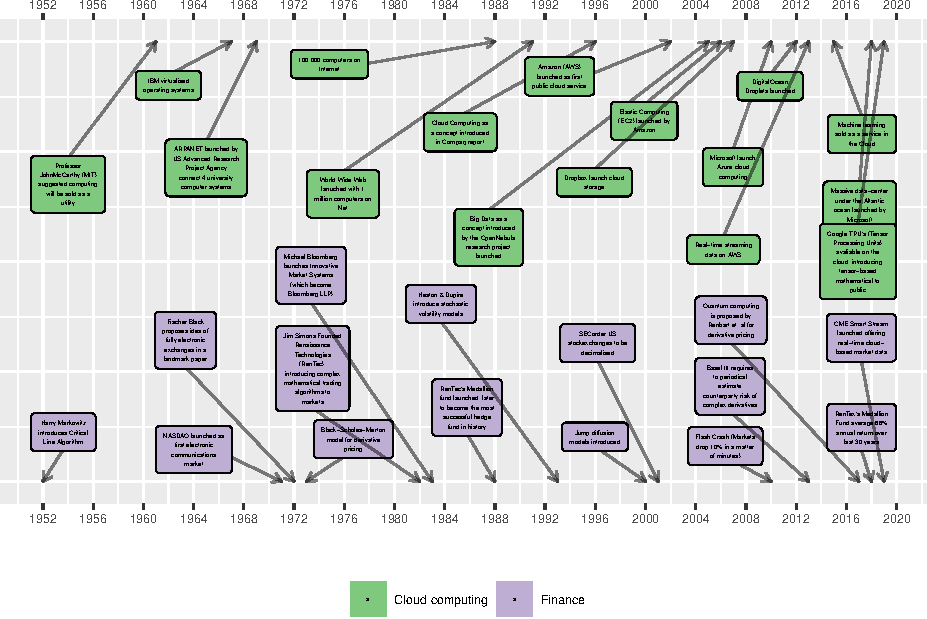
\includegraphics[width=1\linewidth]{qrap_files/figure-latex/timeline-1} 

}

\caption{ Computing landmarks finance and cloud computing.   The data for the cloud computing timeline is sourced from Varghese et al. (2019), while the finance timeline is the authors' calculations}\label{fig:timeline}
\end{figure}

On the \emph{buy-side}, in the early 1950a, Harry Markowitz transforms
quantitative approaches to portfolio management. For example, Markowitz
solved a complex mean-variance portfolio optimisation problem using
algorithmic programming. Meanwhile, in the early 1960s
\href{https://en.wikipedia.org/wiki/Edward_O._Thorp}{Ed Thorp} and
\href{https://en.wikipedia.org/wiki/Jim_Simons_(mathematician)}{John
Simons}, using computer-aided statistical algorithms, showed how
arbitrage opportunities, unseen by traditional hedge fund managers,
could be exploited to beat the market \emph{consistently}.

On the \emph{sell-side} a game-changing breakthrough in the 1970s was a
model to price derivative products (Black and Scholes 1973; Merton 1973)
(BSM model), resulting in the explosive growth of options markets (Cesa
2017). Subsequently, weaknesses in the BSM model fuelled growth in
financial computing. Quantitative researchers, with the increased
availability of computing power, used more realistic continuous-time
pricing models to estimate complex partial differential equations
(Reisinger and Wissmann 2018).

\hypertarget{teaching-environment-for-computing}{%
\section{Teaching environment for
computing}\label{teaching-environment-for-computing}}

Much like teaching statistics and data science, embedding computing in a
financial analytics course has three interconnected teaching advantages:

\begin{enumerate}
\def\labelenumi{\arabic{enumi}.}
\tightlist
\item
  Produce interesting output with data (and code) within the first ten
  minutes of the first class; A have a knock-on effect of challenge
  students to infer meaning from data and statistics from day one;
\item
  Get students to think about computation as an integral part of the
  finance curriculum(Kaplan 2007; Çetinkaya-Rundel and Rundel 2018))
\item
  Demystify the
  \href{https://statmodeling.stat.columbia.edu/2008/05/13/the_folk_theore/}{folk
  theorem of statistical computing} where students think that changing
  the computing environment improves their output;
\end{enumerate}

A standard solution is to use computing labs to facilitate computation
exercises. However, one downside to this approach is that instructors
usually do not have administrative access and therefore struggle to
accomplish basic maintenance tasks, such as pre-loading module-specific
content. Furthermore, this usually leads to a familiar environment for
all courses, rather than specialised setups for more advanced
computational methods. Finally, the most significant downside is that
using computing labs discourages active engagement of computation in all
aspects of the module.

Our approach has been to use a browser-based cloud computing solution to
provide a frictionless student experience in lectures and workshop
sessions. Using the sizeable academic discount, we use the RStudio Teams
enterprise software packages and manage student access using a container
farm of dockerised instances. The Workbench product of the Teams suite
(formerly RStudio server pro) is the web server software that allows
online access to several integrated development environments
(IDEs)\footnote{To date, the software ships with a Launcher package that
  facilitates access to Jupyter notebooks, Jupyterlab, RStudio IDE, and
  Visual Studio} to script in both R and Python (``RStudio Workbench''
2021).

Compared to the computer labs approach, our approach has three distinct
benefits:

The passive lecturing then active labs are replaced by dynamic lectures
and labs and 24/7 access to computing for active independent learning;
Help students who have cost constraints or limitation to accessing
computing hardware; Ease of sharing code, data and environments.

\hypertarget{why-r-and-python}{%
\subsection{Why R and Python?}\label{why-r-and-python}}

R and Python are the two leading languages used in the industry for data
analysis. Thus, to best prepare students to be competitive and perform
on the job market, we made the explicit decision to teach both languages
at master level\footnote{At present, MSc in Quantitative Finance uses
  both languages, and we hope to expand this to all finance programmes
  and the new Actuarial Science masters in the future}. Although some
notable holdouts teach econometrics using commercial graphical user
interfaces(GUI), these languages have infiltrated academia. Proponents
of GUI-based econometrics teaching argue that teaching statistical
concepts is less intimidating to beginners when using a point-and-click
approach than command line methods. Furthermore, the argument goes that
teaching programming and statistics in tandem creates too much friction
for students.

In our experience, such convenience is only possible by removing data
analysis from the course content and providing students with tidy,
rectangular data. But for modern financial data analytics, this approach
is a disservice to students. Furthermore, point-and-click procedures
require a bespoke student user manual that can run to
\href{https://github.com/barryquinn1/FMLmaterial/blob/27d8094fee39fa0284d3a0bfc10e38dcd3bebcac/Introducing\%20Stata.pdf}{40-plus
pages}.

We argue there is a significant learning curve for the novice student,
which isn't generalisable to other analytics workflows. In general,
using a GUI \emph{copy and paste} workflow can increase student
frictions, be more error-prone, be harder to debug, and, most
importantly, disconnect the logical link between computing from
financial analytics(Baumer et al. 2014). But, perhaps most important is
that by learning generalisable coding/data skills, a student an
adequately prepared to into an industry where technologies are rapidly
evolving.

\hypertarget{why-rstudio-teams}{%
\subsection{Why RStudio Teams?}\label{why-rstudio-teams}}

Figure 1 visualises the components that make up the RStudio Team bundle.

\begin{figure}

{\centering 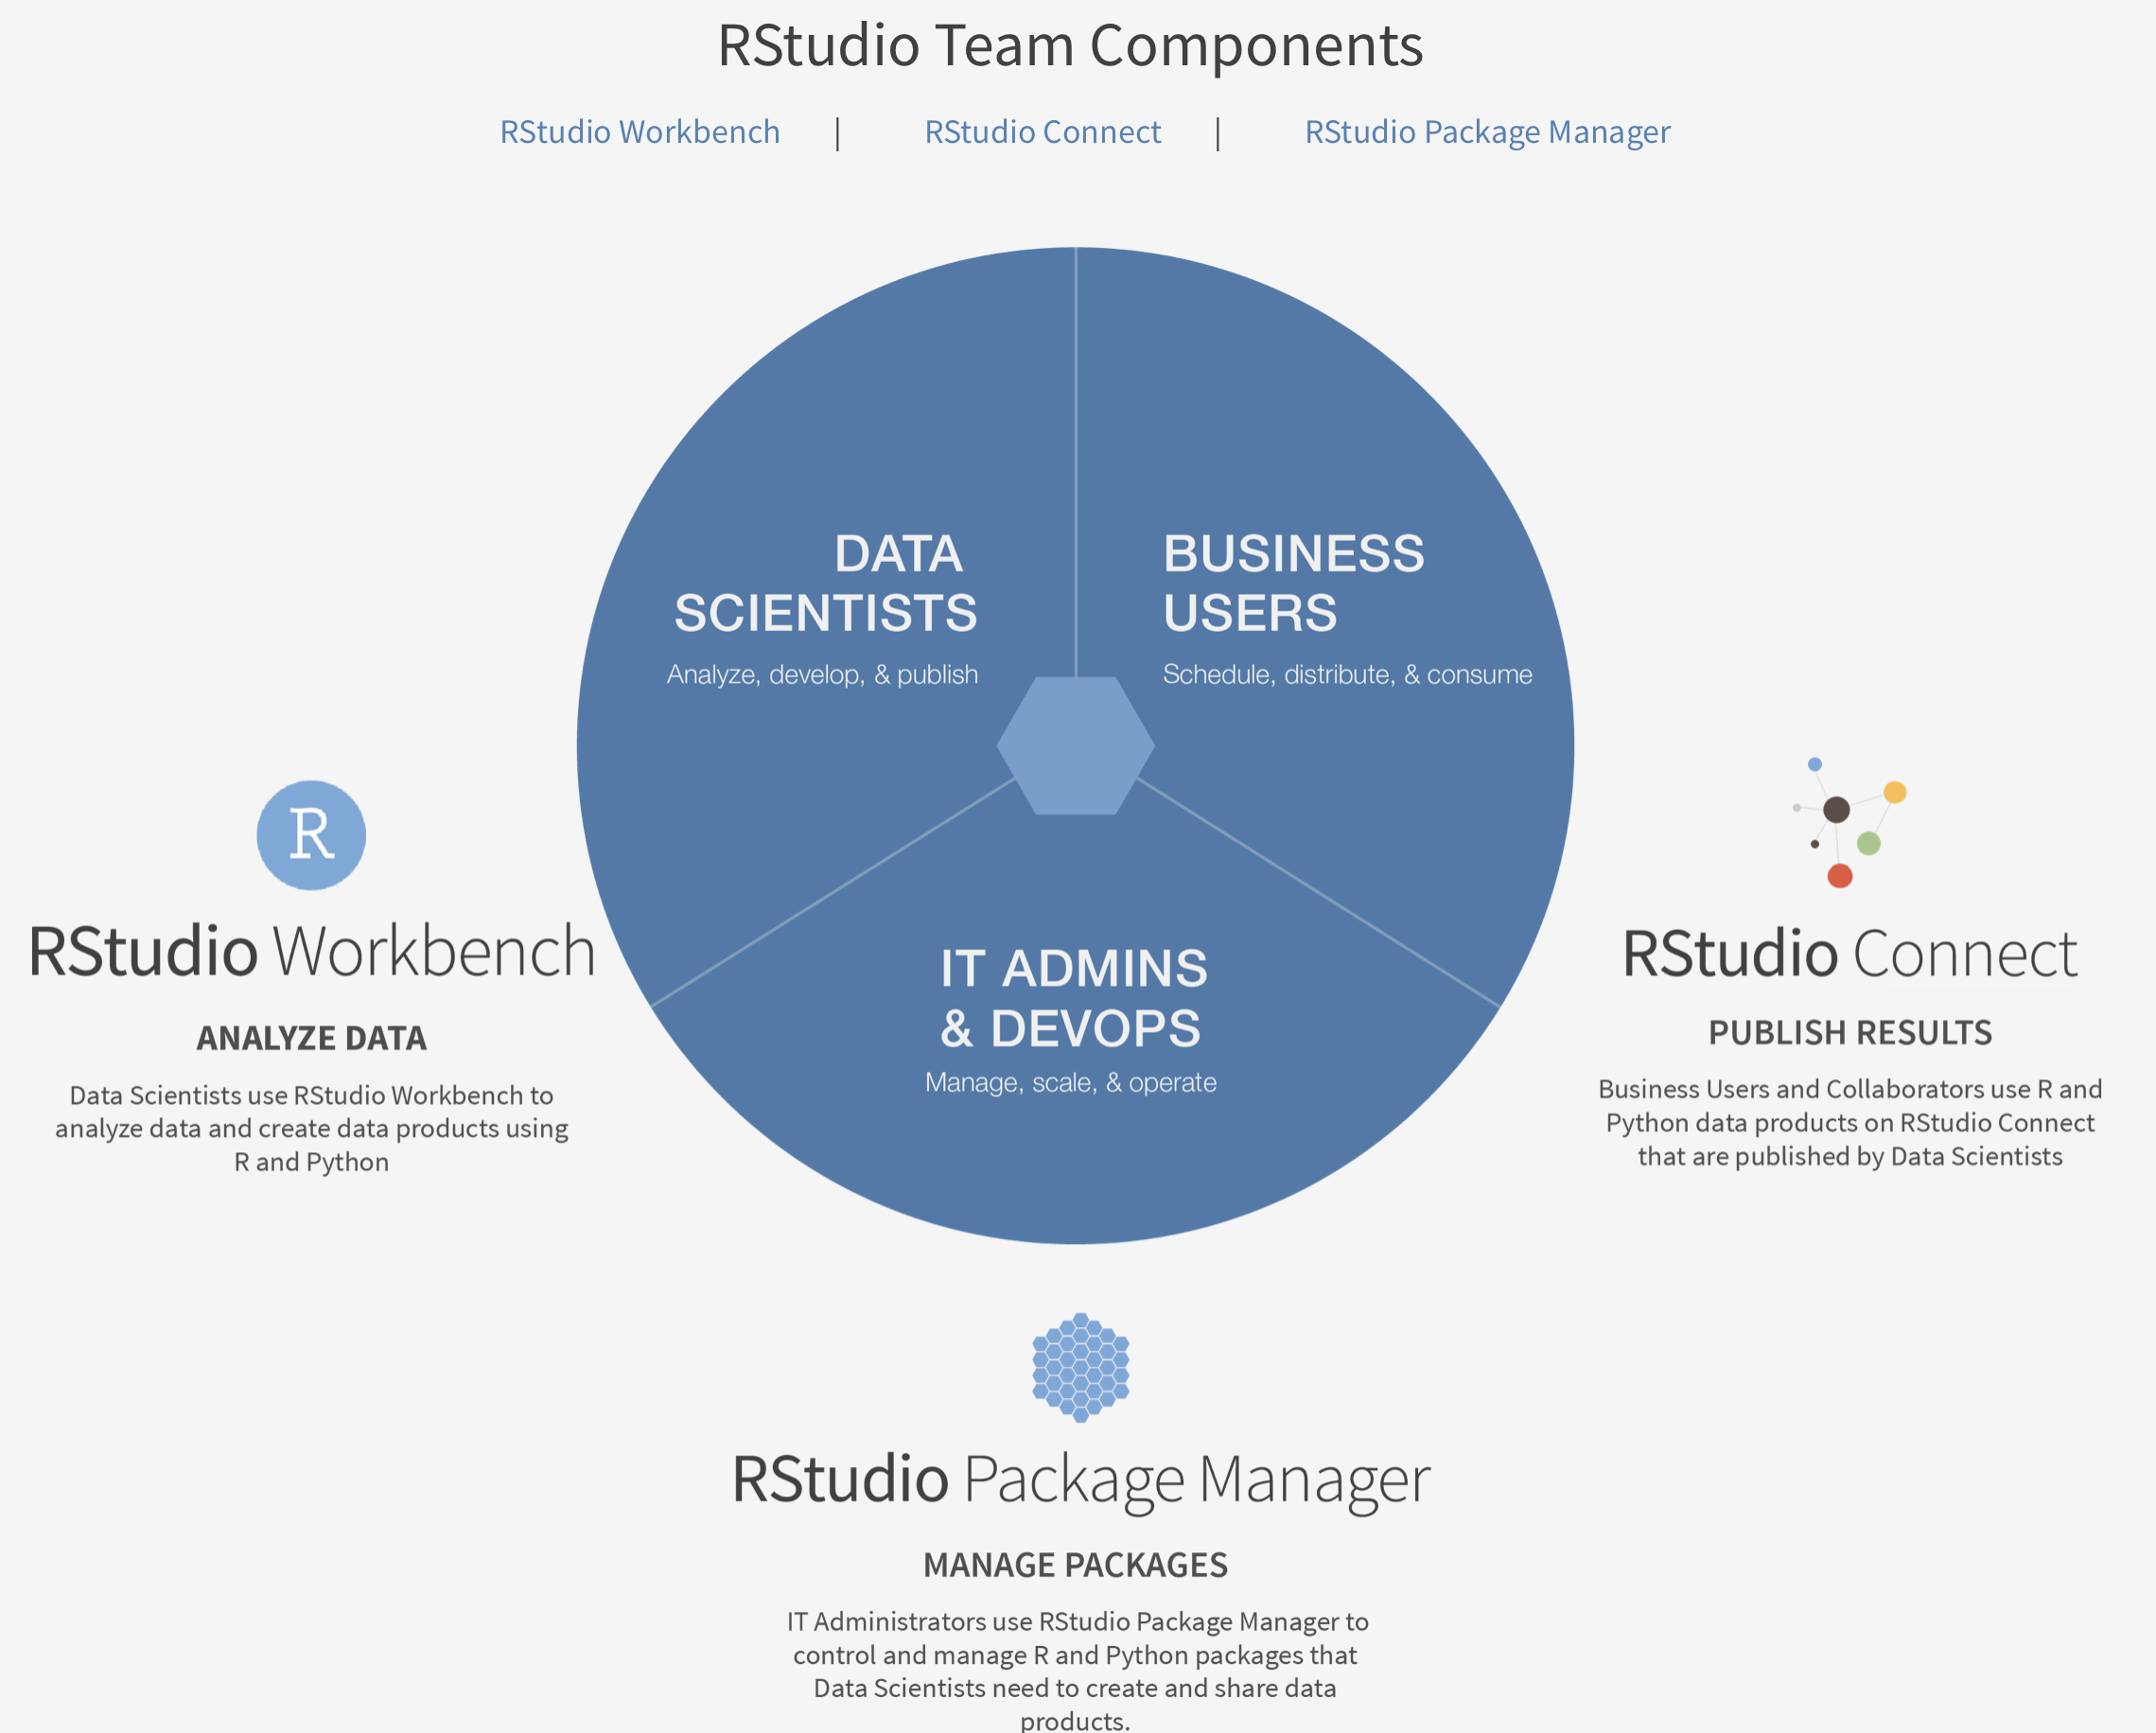
\includegraphics[width=0.7\linewidth]{img/Team} 

}

\caption{The three components of the RStudio Enterprise Team Bundle}\label{fig:rstudioteams}
\end{figure}

RStudio describes this product as follows:

\begin{quote}
RStudio Team is a bundle of RStudio's enterprise-grade professional
software for scaling data science analytical work across your team,
sharing data science results with your key stakeholders, and managing R
and Python packages. RStudio Team includes RStudio Workbench, RStudio
Package Manager, and RStudio Connect. RStudio Team offers convenience,
simplicity, and savings to organisations using R, Python and RStudio at
scale.
\end{quote}

\begin{itemize}
\tightlist
\item
  (``RStudio Team'' 2021)
\end{itemize}

Teams is an enterprise-grade setup offered free of charge for academic
teaching. This discount is a significant saving for educational budgets,
typically between \$15,000 to \$20,000. The School's budget can then
focus on purchasing an agile computing infrastructure.

For teaching computation, the IDE is the most critical tool in this
bundle. The Workbench product comes with Jupyter (notebook and lab) and
RStudio native IDE, which provide a powerful interface that helps
flatten the learning curve in command line teaching. It has a series of
panes to view data, files, and plots interactively. Additionally, since
it is a full-fledged IDE, it also features integrated help, syntax
highlighting, and context-aware tab completion.

Students access the RStudio IDE through a centralised RStudio server
instance, which allows us to provide students with uniform computing
environments. Furthermore, the IDE integrates directly with some
critically essential tools for teaching best practices and reproducible
research, such as R Markdown, Docker, and Git version control.

Importantly, we do not dissuade students from creating local instances
of R and Python, but we do not want it to be a prerequisite of any
module. Students are then allowed to progressively develop their setup
to know that fully-fledged instances are always departmental resources.

\hypertarget{remote-rstudio-workbench-platform}{%
\subsection{Remote RStudio Workbench
Platform}\label{remote-rstudio-workbench-platform}}

A popular approach to running a centralised RStudio server in teaching
computation in higher-level statistics courses is to build a shared
infrastructure with high powered computation power. This hardware is
usually housed securely on-premises and managed by a dedicated IT team.
For example, the Duke University statistics department purchased and
operated a powerful farm of computer servers that can serve
approximately 100 students per semester (Çetinkaya-Rundel and Rundel
2018). We have chosen to run RStudio Workbench using virtualised
hardware on the Microsoft Azure cloud. Figure 3 shows the architecture
of the current setup (without dockerisation). Each student is assigned a
Linux account, authenticated using a departmental login. Students then
connect to a single RStudio Workbench instance, and via the Launcher,
the software can open an IDE to access Python or R scripting
environments. Thus, each student experiences a similar computing
environment solving the perennial.
\href{https://www.kevinwanke.com/why-you-should-never-use-the-phrase-but-it-works-on-my-machine/}{\textbf{but
it worked on my machine?}} problem.

The primary advantage of running and managing a cloud computing platform
is control. Lecturers control a shared user environment for each course,
including required packages, resource configuration, remove or kill
sessions and monitor resource demand on the system. This management work
adds a considerable burden to the lecturer and the IT support, partially
offset by the time saved supporting the build of lab-based PCs. However,
our experience and student feedback suggest that the benefits far
outweigh these additional costs. Furthermore, not providing students
with such a resource is a disservice to their employability in the
modern world of finance.

\begin{figure}

{\centering 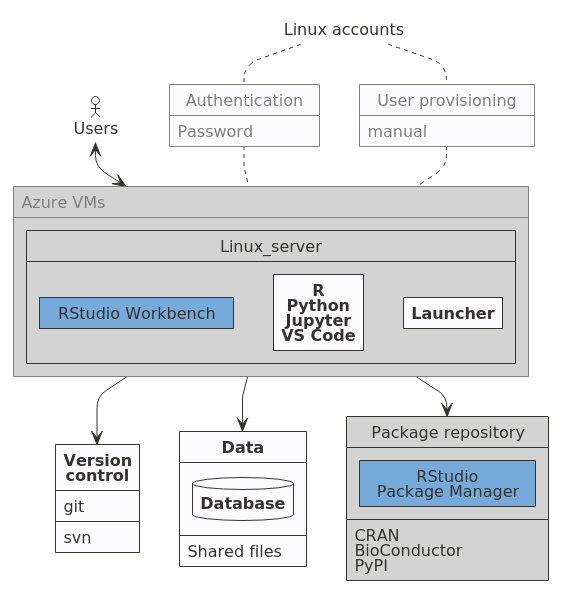
\includegraphics[width=0.7\linewidth]{img/rstudiowb} 

}

\caption{Current set up of RStudio workbench on Azure}\label{fig:current-setup}
\end{figure}

\hypertarget{containerisation-in-finance}{%
\subsection{Containerisation in
finance}\label{containerisation-in-finance}}

Linux containers are technologies that allow you to package and isolate
applications with their entire runtime environment (International Banker
2017). Their strategic advantage is their application independence from
the underlying operating environment enabling standardisation and
automation, significantly lowering cost and operational risk.

Virtualisation technology is the underlying element of cloud computing,
and containers take this to the next level. Cloud computing has
traditionally used virtual machines to distribute available resources
and provide isolated environments among users. The key difference
between virtual machines and containers is that containers share the
same underlying operating system (Mavridis and Karatza 2019)

Containerisation is decades old, but the emergence of the open-source
\href{https://www.ibm.com/cloud/learn/docker}{Docker Engine} has
accelerated the adoption of this technology. Docker is a
\emph{lightweight} virtualisation technology that allows sharing one
operating system so that all code, runtimes, tools, and libraries needed
for a piece of software are made available. This \emph{build once run
anywhere} property makes them highly portable, agile and efficient
approach to running \textbf{sandboxed} instances of RStudio Workbench.
The open-source nature of Docker makes it a transparent and powerful
tool for reproducible computational finance research. From a teaching
perspective, each student can be mapped to a single container, secluding
individual operates and maintaining strict control of computing resource
usages to provide accidental disruption of individual student's work.

Furthermore, clusters can be deployed using a container orchestration
system such as
\href{https://www.ibm.com/cloud/learn/kubernetes}{Kubernetes}, and the
operational overhead can be largely automated using
\href{https://docs.microsoft.com/en-us/azure/aks/intro-kubernetes}{AKS}.
Given they are much lighter weight than VMs, a large container farm of
RStudio instances can be run concurrently on one single server. We plan
to build this infrastructure into our platform and have sketched out the
planned setup in figure 4.

\begin{figure}

{\centering 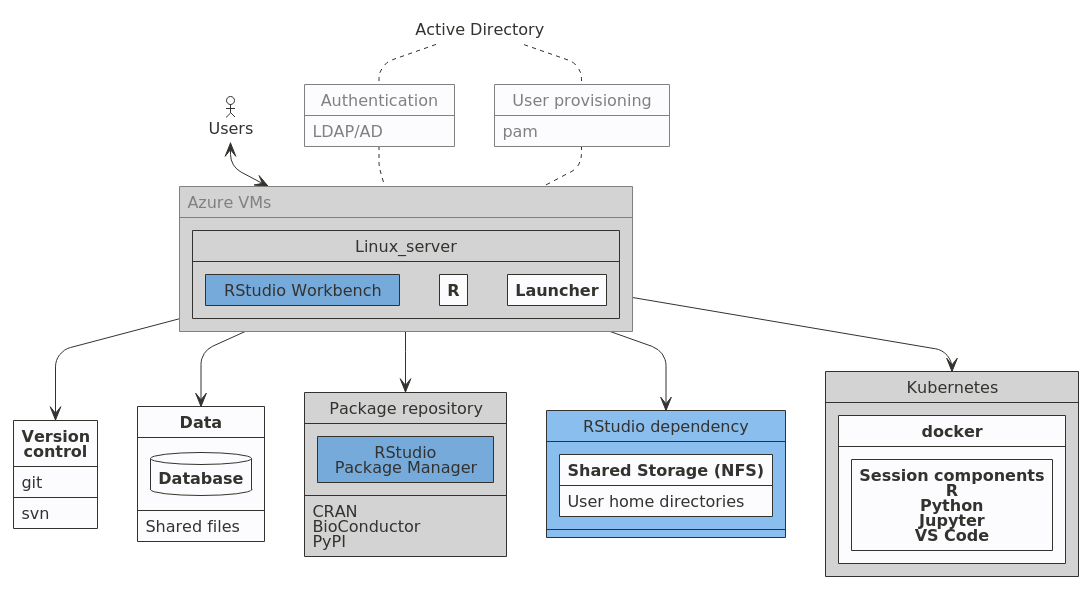
\includegraphics[width=0.8\linewidth]{img/rstudiowb_kb} 

}

\caption{Dockerised set up of RStudio workbench on Azure}\label{fig:future-setup}
\end{figure}

One big challenge with Kubernetes is its steep learning curve, and even
though Azure offers an automating management service, an administrator
will still need to manage individual instance housekeeping. For this
reason, we opted for a more straightforward approach used in Duke
University's statistical department and was created by Mark McCahill. He
kindly shared his setup
(\url{https://gitlab.oit.duke.edu/mccahill/docker-rstudio}), which we
use to create a strict sandboxed virtual environment for each student.

\hypertarget{course-implementation}{%
\section{Course implementation}\label{course-implementation}}

We piloted our new infrastructure at masters level teaching in the
2020-2021 academic year at Queen's Management School. Named Q-RaP
(Queen's management school Remote analytics Platform), students used the
platform in two modules; algorithmic trading and investment and
time-series financial econometrics. Anecdotally, it received excellent
feedback from students, especially when remote teaching and learning was
the norm. In 2021/2022, it will be used in a further two masters level
courses (research methods in finance and computational methods in
finance) and available for some business analytics modules. As well as
the teaching advantages, the resource has the additional benefit of
easing the demand pressures on computer labs.

\hypertarget{reproducibility-with-computational-notebooks}{%
\subsection{Reproducibility with computational
notebooks}\label{reproducibility-with-computational-notebooks}}

Computational notebooks are documents that combine code, discussion and
output in a dynamic reproducible format. An essential advantage of
computational notebooks is that they embody the PPDAC credible analysis
workflow (Problem, Plan, Data, Analysis, Communication). PPDAC is the
professional standard for data analysis and plausible
inference(Spiegelhalter 2019). Unlike the copy and paste approach, all
five parts of the PPDAC approach can be included in one document,
providing an enhanced level of transparency, portability and
reproducibility.

There are two main formats for producing computational notebooks;
Jupyter notebooks and R Markdown. Both are based on Markdown, one of the
most popular markup languages in computing. Using Markdown is different
from using a WYSIWYG editor. In an application like Microsoft Word, you
click buttons to format words and phrases, and the changes are visible
immediately. In contrast, when creating a Markdown-formatted file, you
add Markdown syntax to the text to indicate which words and phrases
should look different. Markdown is highly portable,
platform-independent, future proof, and essential for the modern
financial data scientist.

Out of the box, the Jupyter ecosystem supports python scripting using
the IPython kernel but can support up to 100 different languages (called
`kernels') by installing additional kernels\footnote{\url{https://jupyter4edu.github.io/jupyter-edu-book/jupyter.html}}.
Jupyter notebooks are a lightweight, low learning curve approach to
teaching computing and are an excellent way to get non-technical
students up and running in the first 10 minutes of a course. R Markdown
is probably one of the most powerful tools in the RStudio IDE. R
Markdown files are plain text documents that combine text, code and YAML
metadata into an authoring framework for financial analytics. In the
RStudio IDE, you can open an. Rmd file and working interactively, or
render the file to build a static report or a dynamic web app using the
\texttt{Shiny} packages. For instance, when you render an R Markdown
document, it will combine the text with output from your code. The
rendering process produces static formats such as HTML, pdf and word,
but it can also produce interactive dashboards, web apps, slide shows,
websites and more technical documentation (See video below). We mainly
use Python and R code chunks in our teaching, the former output in the
RStudio environment using the \texttt{reticulate} package.

Pedagogically, the main benefit of R Markdown and Jupyter notebooks is
to embed the logical connection between computing and financial data
analysis. This approach is sometimes referred to as \emph{literate
programming} (Knuth 1984)\footnote{Donald Knuth is pioneering in the
  computing world and create the vastly popular TeX typesetting markup
  language}, which made code, output and narrative inseparable.
Computational notebooks have four advantages over the copy-and-paste
approach:

\begin{enumerate}
\def\labelenumi{\arabic{enumi}.}
\tightlist
\item
  Combining code and output in one document makes it easier for a
  student to locate the source of the errors and encourages more
  experimentation;
\item
  Strict uniformity of the reporting template makes it easier for the
  lecturers to grade;
\item
  Collaboration and group projects become much easier for students when
  using version control. Version control also provides a strict tagging
  system of individual contribution is assessed within a group work
  setting;
\item
  Provides a baseline template document that, as students learn, can be
  more and more lightweight.

  \begin{itemize}
  \tightlist
  \item
    By removing the scaffolding in a slow, piecemeal way as the course
    progresses, active learning appeals.
  \end{itemize}
\end{enumerate}

On balance, using \emph{literate programming} via computational
notebooks has meaningful learning and employability benefits, especially
as it is becoming a standard approach to collaboration in the finance
industry.

\hypertarget{version-control-git-and-github}{%
\subsection{Version control, git and
GitHub}\label{version-control-git-and-github}}

Increasingly, in the world of computational finance, version control is
being used to disseminate and promote innovative coding solutions to
financial problems. Furthermore, in line with applied statistics
curricula (Çetinkaya-Rundel and Rundel 2018), modern finance curricula
should strive to have students produce reproducible output. Git is a
popular command-line version control tool that integrates well with
RStudio Teams. In addition, GitHub is a web-based hosting repository
platform that provides access control and many more collaborative
features to manage teamwork on computing projects.

From a finance industry employability perspective, in the past, there
has been considerable resistance to the user of externally hosted IT
services as security is paramount to highly regulated financial
institutions. The opposition has typically been for strategic and
economic reasons:

\begin{itemize}
\tightlist
\item
  For companies that have swallowed the Windows \emph{Koolaid} there are
  more secure options such as
  \href{https://www.mercurial-scm.org/}{Mercurial}
\item
  It is cheaper for large companies to do it in house
\item
  In a large organisation, there are guaranteed to be fiefs all wanting
  to do things their way and a standardised version control system is
  the only appeal of there is an obvious
  \href{https://www.investopedia.com/terms/t/totalcostofownership.asp}{Total
  Cost of Ownership} benefits. These arguments are now outdated,
  especially with Big Tech acquisition activity in the git ecosystem
  space. For example, in
  \href{https://www.bloomberg.com/news/articles/2018-06-03/microsoft-is-said-to-have-agreed-to-acquire-coding-site-github}{2018},
  Microsoft bought GitHub and soon after
  \href{https://www.bloomberg.com/news/articles/2018-09-19/alphabet-backs-gitlab-s-quest-to-surpass-microsoft-s-github}{Alphabet's
  Google Ventures} took a significant stake in GitLab. This has
  propelled git version control as an industry standard that is now
  easily integrated into all legacy systems, including Windows Servers.
\end{itemize}

Students are required to use git for all assignments in the classroom,
where GitHub is a central repository where students can upload their
work and provide feedback. Recently
\href{https://classroom.github.com/}{GitHub Classroom} was introduced,
providing an enterprise-level service free of charge for academic
teaching.

Before GitHub classrooms, GitHub management tools such as organisation
and teams can be set up privately so that only the students or the group
of students can see and contribute to the assignment. For example, we
used a model where each module has a separate organisation to which
students are invited at the beginning of the semester. For group work,
the teams' tool allows creating a separate team-based repository with
finer-grained access control. In addition, the instructor can monitor
each student's progress and contribution with administrative access
through the continuous integration functionality. GitHub classroom
provides automated instant feedback on simple process tasks, for
example, checking for common reproducibility mistakes in R Markdown
submissions. Feedback on larger prediction projects can be automated
using instant accuracy scores and live leader-boards similar to a Kaggle
contest (Çetinkaya-Rundel and Rundel 2018).

Much of what has been described above has now been automated in GitHub
Classroom and can also be integrated into learning management systems
such as
\href{https://docs.github.com/en/education/manage-coursework-with-github-classroom/teach-with-github-classroom/connect-a-learning-management-system-to-github-classroom}{Canvas}.
The learning curve for these tools is unavoidable. It can be high for
introductory-level courses, but a basic understanding of the workflow in
Figure 5 is sufficient for most modules.

\begin{figure}

{\centering 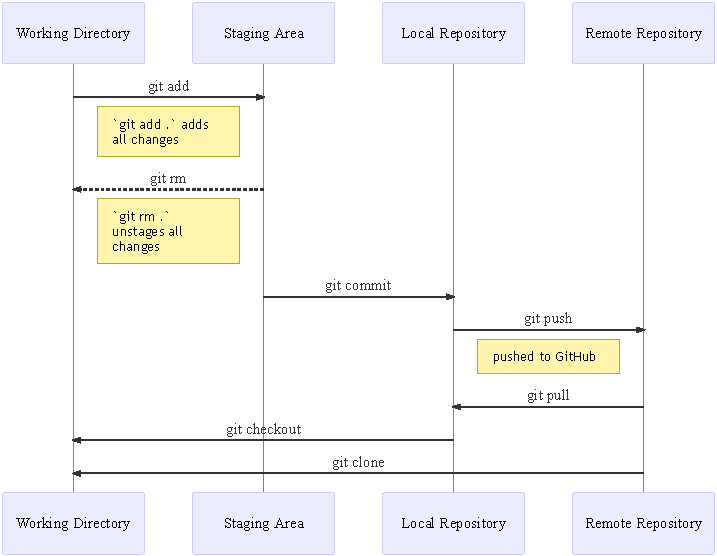
\includegraphics{qrap_files/figure-latex/github-workflow-1} 

}

\caption{Seven git commands students need to learn}\label{fig:github-workflow}
\end{figure}

\hypertarget{discussion}{%
\section{Discussion}\label{discussion}}

As finance educators, our primary objective is to foster industry-ready
graduates for the fast-paced digital age. As we enter a new phase in the
development cycle of financial technology, exposing students to
industry-standard computing technologies is a good start. Our goal with
Q-RaP is to reduce the frictions of teaching computation in finance. Our
vision is to expand this platform to all quantitative modules in the
Management School.

Pedagogically, by embedding computation in a centralised frictionless
way, we can spend more time developing the essential communications
skills for explaining the \emph{why} of the output from the code and
data. Teaching econometrics and statistics in business schools is a
considerable challenge, especially with students from non-technical
backgrounds. The traditional approach off-the-shelf textbook exercises
using mathematical formulas only serves to disenfranchise students from
statistical computing further and is a disservice to the modern business
school graduate. We find the learning curve is significantly flattened
by a code-first approach, increasing student buy-in with approachability
and usability. In addition, mathematical formulas can be introduced to
build a deeper understanding of statistical plumbing and critical
thinking around limitations.

The infrastructure and toolkit we described above ensure buy-in by
making computing a central component of courses and assessments. Using
GitHub as the sole course management tool forces students to become
familiar early, ensuring questions and problems are dealt with at least
before the first assignment date. Furthermore, requiring students to
submit assignments using R Markdown forces students to using a literate
programming approach, ensures reproducibility and embed the PPDAC
principles in their work. Finally, from an employability perspective,
indoctrinating students early with these reproducibility and workflow
principles inoculates any bad computational habits forming, which are
much harder to retrain out of financial researchers.

Importantly, we want to enable students and colleagues to centralise
computation in frictionless and agile education. We hope this can result
in a more meaningful approach to \emph{solving business problems with
data} in a more thoughtful, transparent and significant matter. But,
perhaps most important is that by learning generalisable coding/data
skills, a student an adequately prepared to into an industry where
technologies are rapidly evolving.

\hypertarget{refs}{}
\leavevmode\hypertarget{ref-Apley2020}{}%
Apley, Daniel W, and Jingyu Zhu. 2020. ``Visualizing the Effects of
Predictor Variables in Black Box Supervised Learning Models.'' \emph{J.
R. Stat. Soc. Series B Stat. Methodol.} 82 (4): 1059--86.

\leavevmode\hypertarget{ref-Athey2019b}{}%
Athey, Susan, Mohsen Bayati, Guido Imbens, and Zhaonan Qu. 2019.
``Ensemble Methods for Causal Effects in Panel Data Settings,'' March.
\url{http://arxiv.org/abs/1903.10079}.

\leavevmode\hypertarget{ref-Athey2019a}{}%
Athey, Susan, and Guido W Imbens. 2019. ``Machine Learning Methods That
Economists Should Know About.'' \emph{Annu. Rev. Econom.} 11 (1):
685--725.

\leavevmode\hypertarget{ref-Athey2019c}{}%
Athey, Susan, Julie Tibshirani, and Stefan Wager. 2019. ``Generalized
Random Forests.'' \emph{Aos} 47 (2): 1148--78.

\leavevmode\hypertarget{ref-Athey2017}{}%
Athey, Susan, and Stefan Wager. 2017. ``Policy Learning with
Observational Data,'' February. \url{http://arxiv.org/abs/1702.02896}.

\leavevmode\hypertarget{ref-Bachelier1900}{}%
Bachelier, Louis. 1900. ``Theory of Speculation in the Random Character
of Stock Market Prices.'' \emph{MIT Press, Cambridge, Mass. Blattberg}
1018: 17--78.

\leavevmode\hypertarget{ref-Barredo_Arrieta2020}{}%
Barredo Arrieta, Alejandro, Natalia Diaz-Rodriguez, Javier Del Ser,
Adrien Bennetot, Siham Tabik, Alberto Barbado, Salvador Garcia, et al.
2020. ``Explainable Artificial Intelligence (XAI): Concepts, Taxonomies,
Opportunities and Challenges Toward Responsible AI.'' \emph{Inf. Fusion}
58 (June): 82--115.

\leavevmode\hypertarget{ref-Baumer2014}{}%
Baumer, B, Mine Çetinkaya-Rundel, Andrew Bray, Linda Loi, and N Horton.
2014. ``R Markdown: Integrating a Reproducible Analysis Tool into
Introductory Statistics.'' \emph{Undefined}.

\leavevmode\hypertarget{ref-Black1973}{}%
Black, Fischer, and Myron Scholes. 1973. ``The Pricing of Options and
Corporate Liabilities.'' \emph{J. Polit. Econ.} 81 (3): 637--54.

\leavevmode\hypertarget{ref-Blume2019}{}%
Blume, Jeffrey D, Robert A Greevy, Valerie F Welty, Jeffrey R Smith, and
William D Dupont. 2019. ``An Introduction to Second-Generation
P-Values.'' \emph{Am. Stat.} 73 (sup1): 157--67.

\leavevmode\hypertarget{ref-Breiman2001}{}%
Breiman, Leo. 2001. ``Statistical Modeling: The Two Cultures (with
Comments and a Rejoinder by the Author).'' \emph{Statistical Science} 16
(3): 199--231.

\leavevmode\hypertarget{ref-Cesa2017}{}%
Cesa, Mauro. 2017. ``A Brief History of Quantitative Finance.''
\emph{Probability, Uncertainty and Quantitative Risk} 2 (1): 1--16.

\leavevmode\hypertarget{ref-Chamberlain2000}{}%
Chamberlain, Gary. 2000. ``Econometrics and Decision Theory.'' \emph{J.
Econom.} 95 (2): 255--83.

\leavevmode\hypertarget{ref-Chamberlain2020}{}%
---------. 2020. ``Robust Decision Theory and Econometrics.''
\emph{Annu. Rev. Econom.} 12 (1): 239--71.

\leavevmode\hypertarget{ref-Cunningham2021}{}%
Cunningham, Scott. 2021. \emph{Causal Inference: The Mixtape}. Yale
University Press.

\leavevmode\hypertarget{ref-Cetinkaya-Rundel2018}{}%
Çetinkaya-Rundel, Mine, and Colin Rundel. 2018. ``Infrastructure and
Tools for Teaching Computing Throughout the Statistical Curriculum.''
\emph{Am. Stat.} 72 (1): 58--65.

\leavevmode\hypertarget{ref-Dixon2020}{}%
Dixon, Matthew F, and Nicholas G Polson. 2020. ``Deep Fundamental Factor
Models,'' March. \url{http://arxiv.org/abs/1903.07677}.

\leavevmode\hypertarget{ref-Dreze1972}{}%
Dreze, Jacques H. 1972. ``Econometrics and Decision Theory.''
\emph{Econometrica}.

\leavevmode\hypertarget{ref-Easley2020}{}%
Easley, David, Marcos López de Prado, Maureen O'Hara, and Zhibai Zhang.
2020. ``Microstructure in the Machine Age.'' \emph{Rev. Financ. Stud.},
July.

\leavevmode\hypertarget{ref-Efron2016}{}%
Efron, Bradley, and Trevor Hastie. 2016. \emph{Computer Age Statistical
Inference}. Cambridge University Press.

\leavevmode\hypertarget{ref-Fisher1936}{}%
Fisher, R A. 1936. ``Design of Experiments.'' \emph{Br. Med. J.} 1
(3923): 554--54.

\leavevmode\hypertarget{ref-Gelman2020}{}%
Gelman, Andrew, Jennifer Hill, and Aki Vehtari. 2020. \emph{Regression
and Other Stories}. Cambridge University Press.

\leavevmode\hypertarget{ref-Haavelmo1943}{}%
Haavelmo, Trygve. 1943. ``The Statistical Implications of a System of
Simultaneous Equations.'' \emph{Econometrica} 11 (1): 1--12.

\leavevmode\hypertarget{ref-Hastie2009}{}%
Hastie, Trevor, Robert Tibshirani, and Jerome Friedman. 2009. \emph{The
Elements of Statistical Learning: Data Mining, Inference, and
Prediction, Second Edition}. Springer Science \& Business Media.

\leavevmode\hypertarget{ref-banker2017}{}%
International Banker. 2017. ``The Benefits of Leveraging Containers in
the Financial Services Industry.''
\url{https://internationalbanker.com/technology/benefits-leveraging-containers-financial-services-industry/}.

\leavevmode\hypertarget{ref-IBC2020}{}%
Investment Banking Council. 2020. ``AI in Investment Banking - the New
Frontier.''
\url{https://www.investmentbankingcouncil.org/blog/ai-in-investment-banking-the-new-frontier}.

\leavevmode\hypertarget{ref-Jaeger2021}{}%
Jaeger, Markus, Stephan Krügel, Dimitri Marinelli, Jochen Papenbrock,
and Peter Schwendner. 2021. ``Interpretable Machine Learning for
Diversified Portfolio Construction.'' \emph{The Journal of Financial
Data Science}, June, jfds.2021.1.066.

\leavevmode\hypertarget{ref-Kaplan2007}{}%
Kaplan, Daniel. 2007. ``Computing and Introductory Statistics.''
\emph{Technology Innovations in Statistics Education} 1 (1).

\leavevmode\hypertarget{ref-Knuth1984}{}%
Knuth, D E. 1984. ``Literate Programming.'' \emph{Comput. J.} 27 (2):
97--111.

\leavevmode\hypertarget{ref-Lin2017}{}%
Lin, Sin-Jin, and Ming-Fu Hsu. 2017. ``Incorporated Risk Metrics and
Hybrid AI Techniques for Risk Management.'' \emph{Neural Comput. Appl.}
28 (11): 3477--89.

\leavevmode\hypertarget{ref-Lommers2021}{}%
Lommers, Kristof, Ouns El Harzli, and Jack Kim. 2021. ``Confronting
Machine Learning with Financial Research.'' \emph{The Journal of
Financial Data Science}, June, jfds.2021.1.068.

\leavevmode\hypertarget{ref-De_Prado2019}{}%
López de Prado, Marcos. 2019. ``A Data Science Solution to the
Multiple-Testing Crisis in Financial Research.'' \emph{The Journal of
Financial Data Science} 1 (1): 99--110.

\leavevmode\hypertarget{ref-Lopez_de_Prado2018}{}%
---------. 2018. \emph{Advances in Financial Machine Learning}. John
Wiley \& Sons.

\leavevmode\hypertarget{ref-Mahdavi2020}{}%
Mahdavi, Mehrzad, and Hossein Kazemi. 2020. ``It's All About Data: How
to Make Good Decisions in a World Awash with Information.'' \emph{The
Journal of Financial Data Science} 2 (2): 8--16.

\leavevmode\hypertarget{ref-Mavridis2019}{}%
Mavridis, Ilias, and Helen Karatza. 2019. ``Combining Containers and
Virtual Machines to Enhance Isolation and Extend Functionality on Cloud
Computing.'' \emph{Future Gener. Comput. Syst.} 94 (May): 674--96.

\leavevmode\hypertarget{ref-Merton1973}{}%
Merton, Robert C. 1973. ``Theory of Rational Option Pricing.'' \emph{The
Bell Journal of Economics and Management Science} 4 (1): 141--83.

\leavevmode\hypertarget{ref-Molina2019}{}%
Molina, Mario, and Filiz Garip. 2019. ``Machine Learning for
Sociology.'' \emph{Annu. Rev. Sociol.} 45 (1): 27--45.

\leavevmode\hypertarget{ref-Pearl2009}{}%
Pearl, Judea. 2009. \emph{Causality}. Cambridge University Press.

\leavevmode\hypertarget{ref-Reisinger2018}{}%
Reisinger, Christoph, and Rasmus Wissmann. 2018. ``Finite Difference
Methods for Medium-and High-Dimensional Derivative Pricing PDEs.'' In
\emph{High-Performance Computing in Finance}, 175--95. Chapman;
Hall/CRC.

\leavevmode\hypertarget{ref-RStudioT2021}{}%
``RStudio Team.'' 2021. \url{https://www.rstudio.com/products/team/}.

\leavevmode\hypertarget{ref-RStudioW2021}{}%
``RStudio Workbench.'' 2021.
\url{https://www.rstudio.com/products/workbench/}.

\leavevmode\hypertarget{ref-Rubin1974}{}%
Rubin, Donald B. 1974. ``Estimating Causal Effects of Treatments in
Randomized and Nonrandomized Studies.'' \emph{J. Educ. Psychol.} 66 (5):
688--701.

\leavevmode\hypertarget{ref-SOA2020}{}%
Society of Actuaries. 2020. ``The Powerful Combination of Actuarial
Expertise and InsurTech Knowledge.'' Society of Actuaries;
\url{https://www.soa.org/programs/insurtech/}.

\leavevmode\hypertarget{ref-Spiegelhalter2019}{}%
Spiegelhalter, David. 2019. \emph{The Art of Statistics: Learning from
Data}. Penguin UK.

\leavevmode\hypertarget{ref-Wager2017}{}%
Wager, Stefan, and Susan Athey. 2017. ``Estimation and Inference of
Heterogeneous Treatment Effects Using Random Forests.'' \emph{J. Am.
Stat. Assoc.}, April, 1--15.

\leavevmode\hypertarget{ref-Wolpert1997}{}%
Wolpert, D H, and W G Macready. 1997. ``No Free Lunch Theorems for
Optimization.'' \emph{IEEE Trans. Evol. Comput.} 1 (1): 67--82.

\leavevmode\hypertarget{ref-Wright1934}{}%
Wright, Sewall. 1934. ``The Method of Path Coefficients.'' \emph{Aoms} 5
(3): 161--215.

\leavevmode\hypertarget{ref-Zuo2021}{}%
Zuo, Yi, Thomas G Stewart, and Jeffrey D Blume. 2021. ``Variable
Selection with Second-Generation P-Values.'' \emph{Am. Stat.}, June,
1--21.

\bibliographystyle{unsrt}
\bibliography{biblio.bib}


\end{document}
